\section{Regions of AI:}

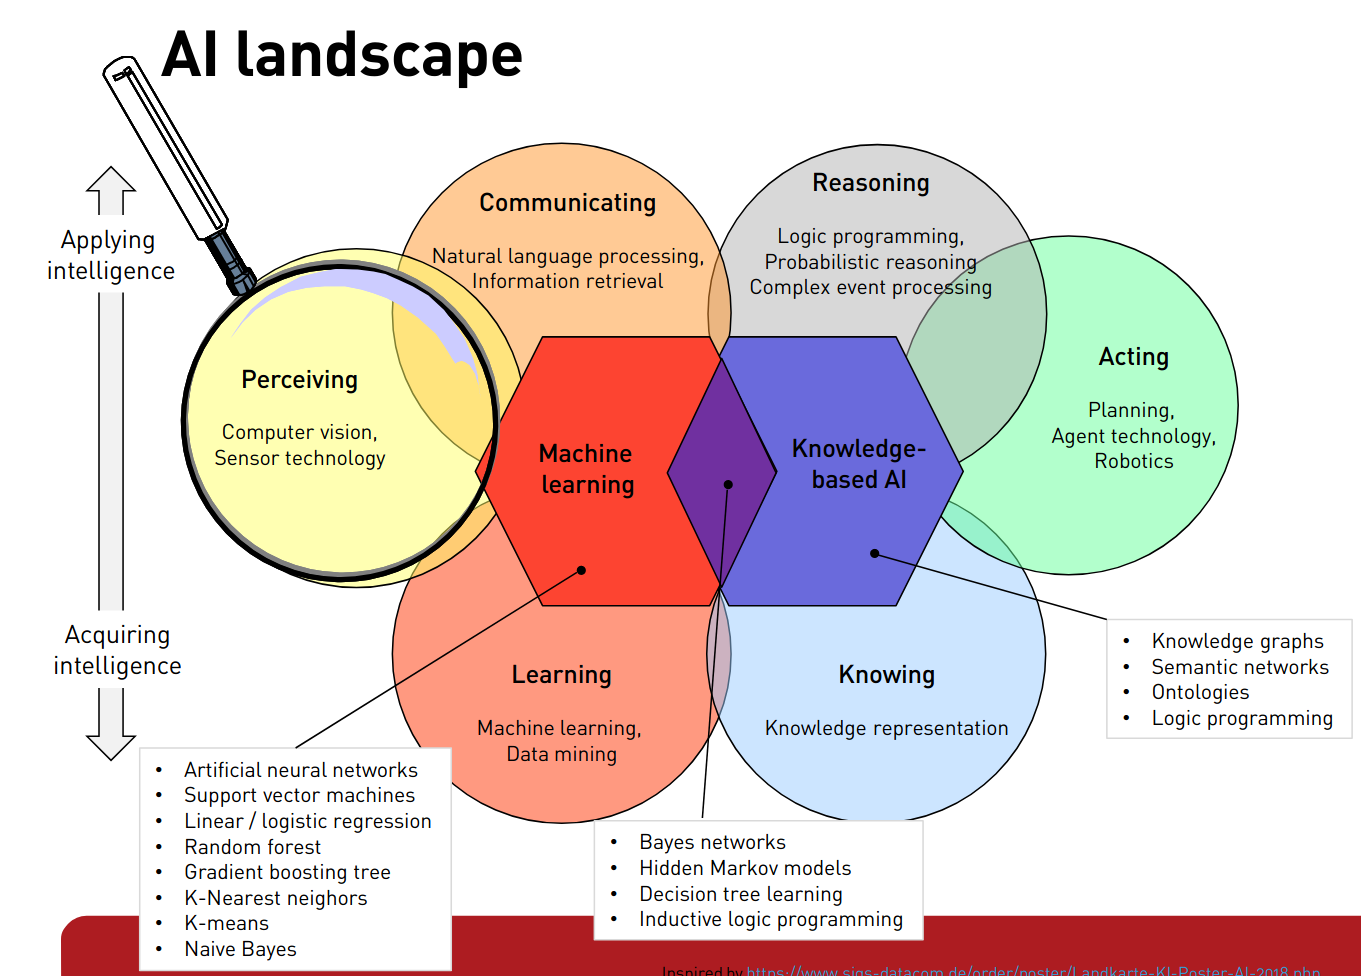
\includegraphics[width=500px]{regrions_of_AI.png}

\section{Machine Learning}

\subsection{Definition}

Machine learning is the approach of generating a model based on inputs (training) and using it for making predictions (productive application) instead of programming instructions explicitly. It is therefore a data-driven approach to finding solutions to problems.

\subsection{Examples of ML tasks}

\begin{itemize}
    \item Spam Filter: Classify emails as spam and not spam
    \item Stock market analysis: Make recommendations on buying or selling stocks
    \item Loyal Customer Detection: Given Data about a customer, classify him/her as loyal or non-loyal customer for the future
\end{itemize}

\subsection{Categories of ML tasks}

\begin{itemize}
    \item Supervised Learning
          \begin{itemize}
              \item Classification
              \item Regression
          \end{itemize}
    \item Unsupervised Learning
          \begin{itemize}
              \item Clustering
              \item Feature selection
              \item Feature extraction
          \end{itemize}
    \item Reinforcement Learning: Try and error mit nach Belohnungsprinzip
\end{itemize}

\subsubsection{Preprocession}

\begin{itemize}
    \item Extracting relevant columns $\rightarrow$
          \begin{itemize}
              \item Faster learning process
              \item better results
          \end{itemize}
    \item Filling missing values
          \begin{itemize}
              \item Deleting rows with missing values
              \item Mean
              \item Median
              \item Use Algorithm that supports missing values
          \end{itemize}
\end{itemize}

\subsubsection{Error functions}

\begin{itemize}
    \item Mean absolute error (MAE)
    \item Mean squared error (MSE)
    \item Rooted MSE (RMSE)
\end{itemize}

\subsubsection{Metrics}

\subsubsection*{Accuracy}

Accuracy answers the question \quotes{\textit{What is the probability that a prediciton is correct?}}.

$$
    Acc = \frac{TP + TN}{TP + TN + FP + FN}
$$

It is only good, if the real distribution of positive and negatives in the data is close to symmetric.

\subsubsection*{Precision}

Precision answers the question \quotes{\textit{If we classify something as positive, how probable is it that it is actually positive?}}.

$$
    Precision = \frac{TP}{TP + FP}
$$

\subsubsection*{Recall}

Recall a.k.a. sensitivity answers the question \quotes{\textit{If a sample is positive, what is the probability we also label it as positive?}}.

$$
    Recall = \frac{TP}{TP + FN}
$$

\subsubsection*{F1 Score}

The F1-score divides the true positives by the sum of the true positives and the mean of the false positives and false negatives. This a high F1-score requires the model to make not few false predictions in either direction. Therefore F1-score is better than accuracy if the real distribution of positive and negative values in the dataset is uneven.

$$
    F1 = 2 \cdot \frac{Precision \cdot Recall}{Precision + Recall} = \frac{TP}{TP + \frac{1}{2} \cdot (FP + FN)}
$$


\subsection*{Validation}

\subsubsection{K-fold cross validation}

\begin{itemize}
    \item split dataset into k subsets
    \item Perform k trainings on k-1 subsets and use the one remaining set for validation such that each subset has been used for validation exactly once
    \item calculate the mean of all k iterations
\end{itemize}

\section{Knowledge Representation}

\subsection{Knowledge Graphs}

A knowledge graph a.k.a. semantic net or ontology is a data structure linking different entities to each other. A common type of knowledge graph is one that consists of triples:

\begin{itemize}
    \item subject: resource
    \item predicate: resource
    \item object: resource or value (string, int, ...)
\end{itemize}

Linked Open Data (LOD) refers to all publicly available data in the internet that can be found using URIs and HTTP.\\
RDF (Resource Description Framework) is a system for describing such data in nets of triples. SPARQL is a query language that can be used to retrieve data from a database which is using the RDF format.\\
A popular free SPARQL server is Apache Jena Fuseki.\\

In the following we can see how to extract tuples (name, country) of city names and country names for which the city is the capital of the country and the country is located in Africa. \lstinline{es} is the prefix for all classes used in this example. \lstinline{cityname}, \lstinline{isCapitalOf}, \lstinline{country} and \lstinline{isInContinent} are classes of predicates. All identifiers starting with a question mark are variables.\\


\begin{lstlisting}[language=SPARQL]
PREFIX ex: <http://example.com/exampleOntology#>
SELECT ?capital
       ?country
WHERE
  {
    # match every city here, assign them to variable ?x and
    # their name and the countries it is a capital for to
    # variables ?capital and ?y
    ?x  ex:cityname       ?capital   ;
        ex:isCapitalOf    ?y         .
    # For all those countries which have capitals,
    # filter those who are in located in Africa and  extract their names
    # concrete values as objects restrict the result set -> conditions
    ?y  ex:countryname    ?country   ;
        ex:isInContinent  ex:Africa  . 
  }
\end{lstlisting}




\subsection{TMDB - The movie database}

Popular collaborative database of movies with the following entities:

\begin{itemize}
    \item Movie
    \item Country
    \item Company
    \item Genre
    \item Collection
    \item Keyword
    \item Cast
    \item Crew
    \item Language
\end{itemize}

\section{Natural Language Processing (NLP)}

\subsection{Areas of NLP}

\begin{itemize}
    \item \textbf{Information retrieval:} Retrieving relevant information from documents e.g. by using SPARQL-queries.
    \item \textbf{Text classification}
    \item \textbf{Information Extraction:} Building knowledge graphs from natural language texts
    \item \textbf{Question Answering:} Answering natural language questions like \quotes{What is the weather todoay?}
    \item \textbf{Machine Translation:} translating a text into a different language
    \item \textbf{Text Generation:} Generate natural language texts e.g. answers to natural language questions for a voice assistant.
\end{itemize}

\subsection{SpaCy - NLP library}

\begin{itemize}
    \item \textbf{Tokenization:} Segmenting a text into single words punctuation marks etc.
    \item \textbf{Part-of-speech (POS) tagging:} Assigning word types to tokens like verb, noun, adjective...
    \item \textbf{Dependency Parsing:} Assigning dependency syntactic labels describing the relations between tokens e.g. subject, object, predicate
    \item \textbf{Lemmatization:} Finding the base form of words e.g. drives $rightarrow$ drive
    \item \textbf{Sentence Boundary Detection (SBD):} Splitting text by sentences. This is not Trivial as full stops can also appear mid-sentence e.g. when writing acronyms.
    \item \textbf{Named Entity Recognition (NER):} Labelling real world objects like persons, companies or locations
    \item \textbf{Entity Linking (EL):} Linking tokens or groups of tokens in a text to unambiguous entries in a knowledge base e.g. a knowledge graph.
    \item \textbf{Similarity:} Calculating similarity of words or text spans
    \item \textbf{Classification:} Assigning categories or labels to a whole document or parts of a document
    \item \textbf{Rule-based Matching:} Finding sequences of tokens based on their linguistic annotations similar to regular expressions.
    \item \textbf{Training:} Updating and improving a statistical model's prediction
    \item \textbf{Serialization:} Saving objects to files or byte strings
\end{itemize}

\subsubsection*{A simple idea for implementing Question Answering with SpaCy:}
If we already have a database with questions and their answers we can answer new questions by returning the answer to the most similar question in our database.

\subsection{Bag-Of-Words}

Bag of words is a dictionary mapping each unique word to the number of occurrences. This dictionary can be used as an input for ML models.

Advantages: simplicity\\
Disadvantages: no information about grammar and relation of words, too high focus on stop words, big vector if many words are used which might be too small for supervised ML

\subsection{tf-idf}
Term frequency - inverse document frequency\\
$$
    \frac{occurence count of word}{average occurence count of word in general}
$$

The result is that stop words are only taken into account if they appear more often then usual.

\subsection{n-gram model}

Using n-gram model with n=1 is equal to using the bag-of-words model. N-gram groups n words together in an overlapping fashion. This way we hope to extract some grammar information and relation between words from the text. However this also increases the size of of the input vectors for ML models




\section{Computer Vision}

\subsection{Common Types of Applications}

\begin{itemize}
    \item \textbf{Optical Character Recognition (OCR):}
          \\Input: Image of handwritten or typewritten text.\\
          Output: Text Document
          \begin{itemize}
              \item Digitalization of documents
              \item Scanning addresses on letters
              \item Evaluating forms
          \end{itemize}
    \item \textbf{Face Recognition:}\\
          Input: Image\\
          Output: Information about face: position and maybe building on top of that further information in form of classification
          \begin{itemize}
              \item Autotagging camera images
              \item Image search
              \item Detecting people on security cameras
          \end{itemize}
    \item \textbf{Medical Applications:} Detecting anomalies in CT/ MRI / Ultrasound images
    \item \textbf{Industrial / Agricultural Applications:}
          \begin{itemize}
              \item Sorting fruits in agriculture
              \item Quality management
              \item Automation of manufacturing process using robots with computer vision technologies
          \end{itemize}
    \item \textbf{Military Applications:}
          \begin{itemize}
              \item Detection of enemies
              \item Missile guidance
              \item Autonomous drones and vehicles
          \end{itemize}
    \item \textbf{Automotive Applications:}
          \begin{itemize}
              \item Collision warning
              \item Parking aid
              \item Road sign detection
              \item Autonomous driving
          \end{itemize}
    \item \textbf{Cinema:}
          \begin{itemize}
              \item Motion Capturing: translating real world motion into the motions of animated movie characters
          \end{itemize}
\end{itemize}

\section{AI application development}

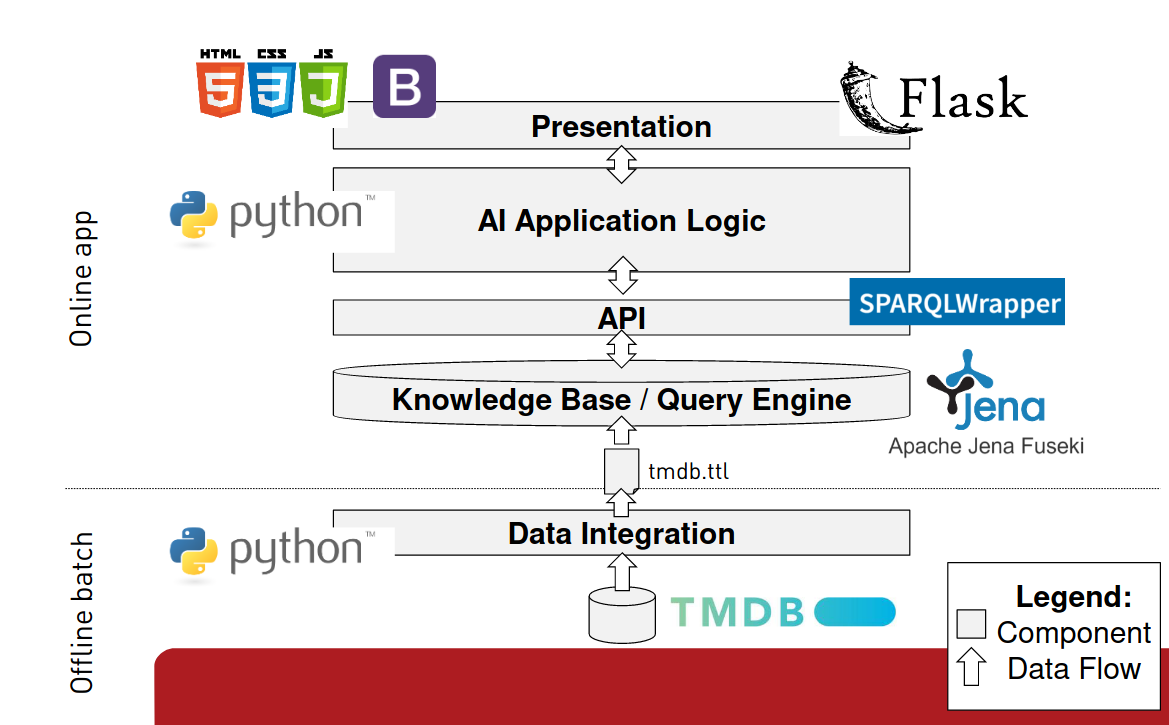
\includegraphics[width=400px]{AI_application_dev.png}

In the following we will list some common tools for application development:

\begin{itemize}
    \item \textbf{Flask:} Micro web framework written in Python.
    \item \textbf{Jinja:} Web template engine for Python. Similar to Django but provides Python-like expressions while ensuring that templates are evaluated in a sandbox. In essence it evaluates HTML with embedded Python.
    \item \textbf{Bootstrap:} CSS-Framework mit SCC und HTML Gestaltungsvorlagen, die durch anhängen von Tags and das HTML des Benutzers verwendet werden können.
\end{itemize}

\section{Ethical Aspects of AI}

\subsubsection*{Hype}

There was a hype around artificial intelligence which lead to exaggerated opinions and crazy movies:

\begin{itemize}
    \item Marvin Minsky 1970: \quotes{Within 10 years computers won't even keep us as pets.}
    \item Ray Kurzweil 2005: \quotes{Artificial Intelligence will reach human levels by around 2029. Follow that out further to, say, 2045 we will have multiplied the intelligence the human biological machine intelligence of our civilization a billion-fold.}
\end{itemize}

\subsubsection*{Reality}

In reality AI applications are ambiguous and used in a lot of day to day situations. However, they are specialized in certain areas and are not even close to being as intelligent as humans.

\subsubsection*{Cyborg - Technological enhancement of human body}

\begin{itemize}
    \item Neil Harbisson with an Antenna allowing him to perceive colors that go beyond human perception.
    \item Amanda Kitts with an arm prosthesis
    \item Hearing aid
    \item Heart pacemaker
\end{itemize}

\subsubsection*{Industry 4.0 replacing human labor}

In fact there have been multiple industrial revolutions before. Now we are at the point that machine learning applications are capable of replacing some human labor. This has positive and negative effects on society. People will loose their jobs. But this also means that there is less labor needed, which is a good thing and can lead to an overall increasing standard of living.

\subsubsection*{Biased Machine Learning}

Machine Learning models can not be better than the data they are trained on. That means if we have biased data supporting stereotypes, then we will face the problem that machine learning models decisions are also driven by those stereotypes.

\subsubsection*{Decision Making}

Is it ethically correct to let machine learning models take decisions even if it has been shown that the divisions are more accurate than human decisions in some cases?\\
Examples are:

\begin{itemize}
    \item Autonomous driving and accidents
    \item Choosing employees for a company based on features of the applicants
    \item High frequency trading
\end{itemize}


\section{CEP - Complex Event Processing}

Complex Event Processing ist ein Themengebiet der Informatik, das sich mit der Erkennung, Analyse und Verarbeitung voneinander abhängiger Ereignisse beschäftigt.

\subsection{CEP Application Examples}

\begin{itemize}
    \item \textbf{Fraud Detection:}\\
          Input: Stream of Credit Card Transactions\\
          Output: Fraud alert triggering a human interview
    \item \textbf{Predictive Maintenance:}\\
          Input: Stream of Sensor inputs from machinery in factory\\
          Analysis: Check for patterns that indicate deterioration of machine e.g. vibration\\
          Output: Warning triggering soon replacement of the machine part
    \item \textbf{Logistics:}\\
          Input: Stream of RFID signals\\
          Analysis: Check for conditions that require certain actions\\
          Output: Trigger actions such as inform logistic partners, inform customers about delivery, alert
    \item \textbf{Stock Market Trading:}\\
          Input: Stream of stock market data\\
          Output: Sell or buy decision
\end{itemize}

\subsection{Terminology}

\subsubsection*{Definition CEP}

Processing streams of event data and deriving conclusions from them.

\subsubsection*{Definition Event}

Something notable that happens in real life.

\subsubsection*{Definition Event Object}

A data record representing a single event.

\subsubsection*{Event Type}

Specifies the common structure for event objects such as their attributes and data types. Therefore it is a class and event objects are instances of it.

\subsubsection*{DBMS vs CEP}

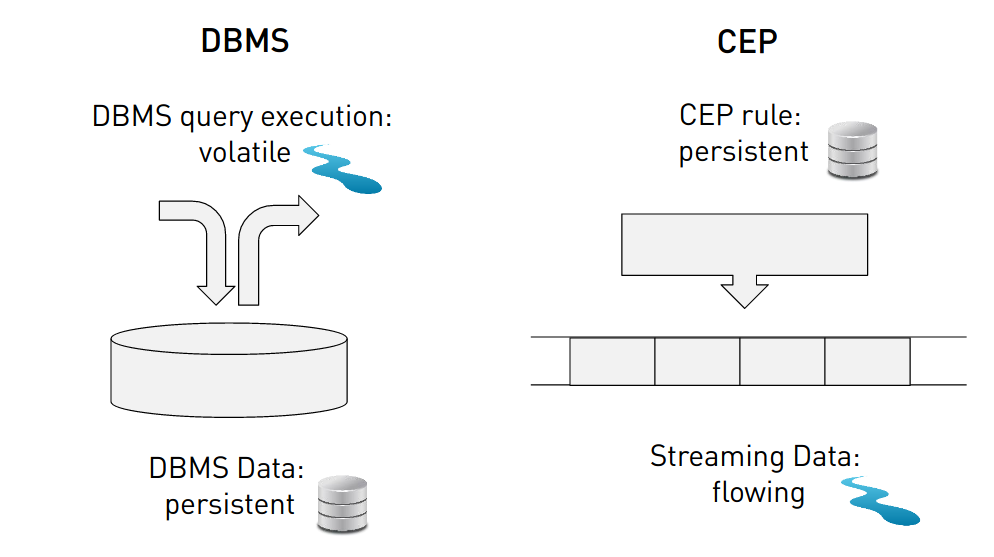
\includegraphics[width=500px]{dbms_vs_cep.png}

\subsection{Sliding Window}

A sliding window is a method for repeatedly capturing sequences of information from an event data stream from the near past. We define a window with duration/size $n$ (captures all data in the last $n$ seconds) and a windowing frequency $m$ (captures the last $n$ seconds every $m$ seconds).

\subsection{Types of CEP rules}

\begin{itemize}
    \item \textbf{Filtering:} Using reg ex
    \item \textbf{Pattern matching:} Detecting successions of events e.g. [sign up].next([use sign up discount code]).next([buy]).next([cancel account]). May be used for the generation of the event: [sneaky customer]
    \item \textbf{Value progression analysis:} Using e.g. sliding window to detect changes in values over time. E.g. a drop of 100km/h of a car in 5 seconds might detect a [car crash] event.
    \item \textbf{Time Progression analysis:} The time span in which event data is read is analysed as opposed to their values. E.g. if we do not get a heart break signal for over 1 minute we raise the event [just passed by :(]
    \item \textbf{Semantic Enrichment / Iterative CEP:} Applying rules for CEP from low level to high level can lead to extracting semantic information in form of higher level events.
\end{itemize}

\subsection{CEP Technology}

\begin{itemize}
    \item Apache Kafka
    \item Apache Flink
    \item Apache Spark
    \item Drools Fusion
    \item MS Azure Stream Analytics
    \item Oracle Stream Analytics
    \item SAG Apama
    \item SAP ESP
    \item TIBCO
    \item IBM WebSphere Business Events
\end{itemize}

